\documentclass{article}
\usepackage{tikz}
\usepackage{pgfplots}
\usepackage{amsmath}
\pgfplotsset{compat=1.18}
\usepackage{geometry}
\geometry{a4paper, margin=1cm} 

\begin{document}

\begin{center}
\section*{Visualizing Normal Distributions Transform (NDT) Steps (TikZ Series)}
\end{center}

\vspace{0.5cm}

% --- FIGURE 1: Space Subdivision & Voxel Grid ---
\begin{figure}[htbp]
\centering
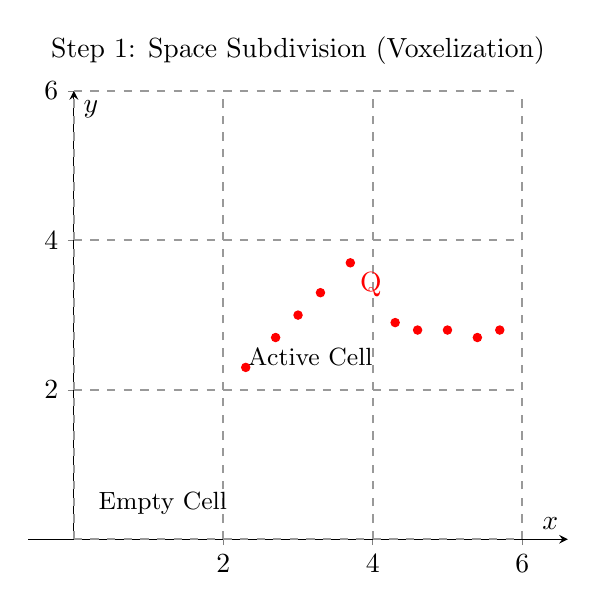
\begin{tikzpicture}
\begin{axis}[
    axis lines=middle,
    xmin=0, xmax=6, ymin=0, ymax=6,
    xtick={0, 2, 4, 6}, ytick={0, 2, 4, 6},
    axis equal, 
    xlabel=$x$, ylabel=$y$,
    title={Step 1: Space Subdivision (Voxelization)},
    grid=none
]

% Draw Voxel Grid (2x2 cells)
\draw[black!40!white, dashed, thick, step=2] (0,0) grid (6,6);

% Target Point Cloud Q (red, clustered in certain cells)
% Cell (2,2) to (4,4) - Diagonal cluster
\addplot[mark=*, red, only marks, mark size=1.5pt] coordinates {(2.3, 2.3) (2.7, 2.7) (3.0, 3.0) (3.3, 3.3) (3.7, 3.7)} node[anchor=north west] at (3.7, 3.7) {Q};
% Cell (4,2) to (6,4) - Horizontal cluster
\addplot[mark=*, red, only marks, mark size=1.5pt] coordinates {(4.3, 2.9) (4.6, 2.8) (5.0, 2.8) (5.4, 2.7) (5.7, 2.8)};
% Cell (0,0) to (2,2) - Empty
% Cell (2,0) to (4,2) - Empty

\node[font=\small, anchor=south west] at (0.2, 0.2) {Empty Cell};
\node[font=\small, anchor=south west] at (2.2, 2.2) {Active Cell};

\end{axis}
\end{tikzpicture}
\caption{Step 1: The target point cloud (Q) is placed into a regular spatial grid (voxels in 3D, squares in 2D). Cells with fewer than a minimum number of points (e.g., 3 points) are usually ignored to prevent mathematical instability.}
\label{fig:voxelization}
\end{figure}

\vspace{0.5cm}

% --- FIGURE 2: Calculating PDFs (Normal Distributions) ---
\begin{figure}[htbp]
\centering
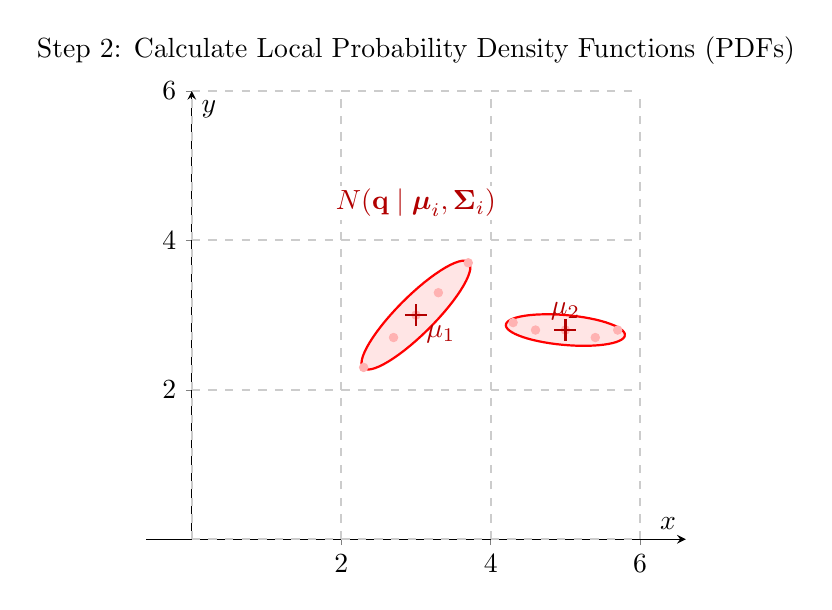
\begin{tikzpicture}
\begin{axis}[
    axis lines=middle,
    xmin=0, xmax=6, ymin=0, ymax=6,
    xtick={0, 2, 4, 6}, ytick={0, 2, 4, 6},
    axis equal, 
    xlabel=$x$, ylabel=$y$,
    title={Step 2: Calculate Local Probability Density Functions (PDFs)},
    grid=none
]

% Draw Voxel Grid
\draw[black!20!white, dashed, thick, step=2] (0,0) grid (6,6);

% Q points (faint for context)
\addplot[mark=*, red!30!white, only marks, mark size=1.5pt] coordinates {(2.3, 2.3) (2.7, 2.7) (3.0, 3.0) (3.3, 3.3) (3.7, 3.7) (4.3, 2.9) (4.6, 2.8) (5.0, 2.8) (5.4, 2.7) (5.7, 2.8)};

% Covariance Ellipse 1 (Cell 2,2 to 4,4): Mean (3,3), rotated 45 deg
% Parametric equation for rotated ellipse: x = h + a*cos(t)*cos(ang) - b*sin(t)*sin(ang), y = k + a*cos(t)*sin(ang) + b*sin(t)*cos(ang)
\addplot[red, thick, domain=0:360, samples=60, fill=red!20!white, fill opacity=0.5] 
    ({3 + 1.0*cos(x)*cos(45) - 0.25*sin(x)*sin(45)}, 
     {3 + 1.0*cos(x)*sin(45) + 0.25*sin(x)*cos(45)});
\addplot[mark=+, red!70!black, mark size=4pt, thick] coordinates {(3,3)} node[anchor=north west] {\(\mu_1\)};

% Covariance Ellipse 2 (Cell 4,2 to 6,4): Mean (5,2.8), rotated -5 deg
\addplot[red, thick, domain=0:360, samples=60, fill=red!20!white, fill opacity=0.5] 
    ({5 + 0.8*cos(x)*cos(-5) - 0.2*sin(x)*sin(-5)}, 
     {2.8 + 0.8*cos(x)*sin(-5) + 0.2*sin(x)*cos(-5)});
\addplot[mark=+, red!70!black, mark size=4pt, thick] coordinates {(5,2.8)} node[anchor=south] {\(\mu_2\)};

\node[red!70!black, fill=white, inner sep=1pt] at (3, 4.5) {\(N(\mathbf{q} \mid \boldsymbol{\mu}_i, \boldsymbol{\Sigma}_i)\)};

\end{axis}
\end{tikzpicture}
\caption{Step 2: For every active cell, the sample mean (\(\boldsymbol{\mu}_i\)) and covariance matrix (\(\boldsymbol{\Sigma}_i\)) of the target points are calculated. This transforms the discrete point cloud into a piecewise continuous set of multi-variate Gaussian probability distributions (represented here by covariance ellipses).}
\label{fig:pdfs}
\end{figure}

\vspace{0.5cm}

% --- FIGURE 3: Mapping the Source Cloud ---
\begin{figure}[htbp]
\centering
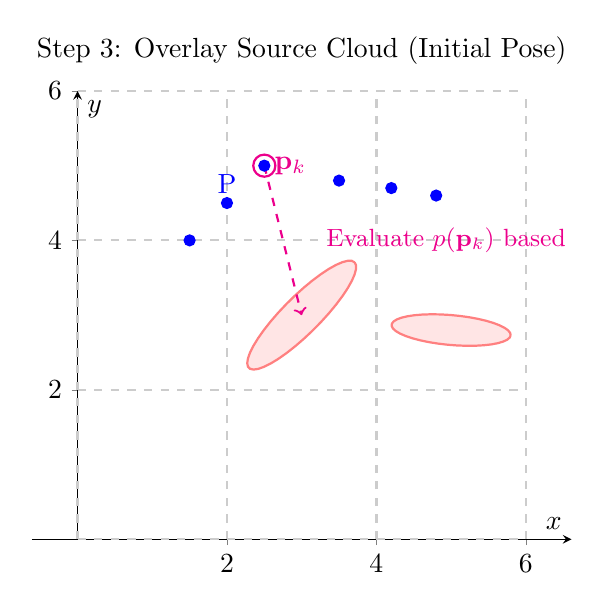
\begin{tikzpicture}
\begin{axis}[
    axis lines=middle,
    xmin=0, xmax=6, ymin=0, ymax=6,
    xtick={0, 2, 4, 6}, ytick={0, 2, 4, 6},
    axis equal, 
    xlabel=$x$, ylabel=$y$,
    title={Step 3: Overlay Source Cloud (Initial Pose)},
    grid=none
]

% Voxel Grid & Ellipses (Background)
\draw[black!20!white, dashed, thick, step=2] (0,0) grid (6,6);
\addplot[red!50!white, thick, domain=0:360, samples=40, fill=red!10!white] 
    ({3 + 1.0*cos(x)*cos(45) - 0.25*sin(x)*sin(45)}, {3 + 1.0*cos(x)*sin(45) + 0.25*sin(x)*cos(45)});
\addplot[red!50!white, thick, domain=0:360, samples=40, fill=red!10!white] 
    ({5 + 0.8*cos(x)*cos(-5) - 0.2*sin(x)*sin(-5)}, {2.8 + 0.8*cos(x)*sin(-5) + 0.2*sin(x)*cos(-5)});

% Source Point Cloud P (blue, misaligned)
\addplot[mark=*, blue, only marks, mark size=2pt] coordinates {(1.5, 4.0) (2.0, 4.5) (2.5, 5.0)} node[anchor=south] at (2.0, 4.5) {P};
\addplot[mark=*, blue, only marks, mark size=2pt] coordinates {(3.5, 4.8) (4.2, 4.7) (4.8, 4.6)};

% Highlight one point mapping to a cell
\addplot[mark=o, magenta, mark size=4pt, thick] coordinates {(2.5, 5.0)} node[anchor=west] {\(\mathbf{p}_k\)};
\draw[->, magenta, thick, dashed] (2.5, 5.0) -- (3, 3);
\node[magenta, font=\small, anchor=west] at (3.2, 4) {Evaluate \(p(\mathbf{p}_k)\) based on Cell 1};

\end{axis}
\end{tikzpicture}
\caption{Step 3: The source point cloud (P) is projected into the voxel grid using its initial, unoptimized transformation. We determine which spatial cell each source point falls into (or its nearest neighbors if using smoothed NDT).}
\label{fig:source_mapping}
\end{figure}

\vspace{0.5cm}

% --- FIGURE 4: NDT Score Formulation (Zoomed) ---
\begin{figure}[htbp]
\centering
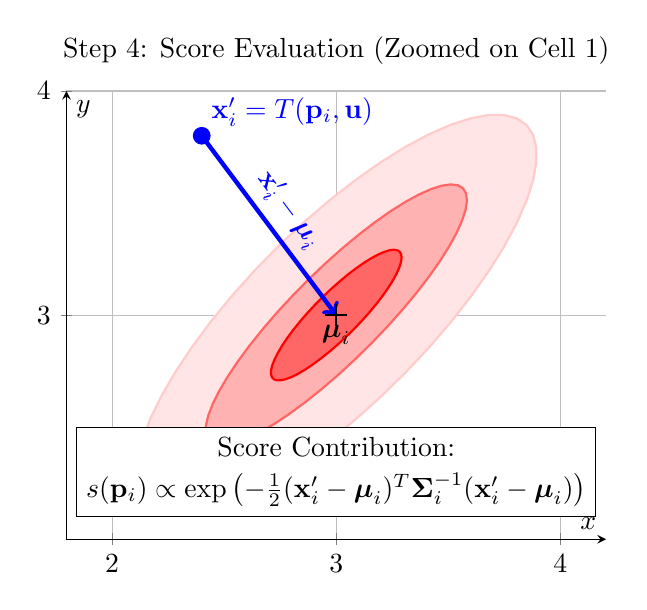
\begin{tikzpicture}
\begin{axis}[
    axis lines=middle,
    xmin=2, xmax=4, ymin=2, ymax=4,
    xtick={2, 3, 4}, ytick={2, 3, 4},
    axis equal,
    xlabel=$x$, ylabel=$y$,
    title={Step 4: Score Evaluation (Zoomed on Cell 1)},
    grid=both
]

% Show nested ellipses to represent density decay
\addplot[red!20!white, thick, domain=0:360, samples=50, fill=red!10!white] 
    ({3 + 1.2*cos(x)*cos(45) - 0.4*sin(x)*sin(45)}, {3 + 1.2*cos(x)*sin(45) + 0.4*sin(x)*cos(45)}); % 2 sigma
\addplot[red!60!white, thick, domain=0:360, samples=50, fill=red!30!white] 
    ({3 + 0.8*cos(x)*cos(45) - 0.2*sin(x)*sin(45)}, {3 + 0.8*cos(x)*sin(45) + 0.2*sin(x)*cos(45)}); % 1 sigma
\addplot[red, thick, domain=0:360, samples=50, fill=red!60!white] 
    ({3 + 0.4*cos(x)*cos(45) - 0.1*sin(x)*sin(45)}, {3 + 0.4*cos(x)*sin(45) + 0.1*sin(x)*cos(45)}); % 0.5 sigma

\addplot[mark=+, black, mark size=4pt, thick] coordinates {(3,3)} node[anchor=north] {\(\boldsymbol{\mu}_i\)};

% Source Point
\addplot[mark=*, blue, only marks, mark size=3pt] coordinates {(2.4, 3.8)} node[anchor=south west] {\(\mathbf{x}_i' = T(\mathbf{p}_i, \mathbf{u})\)};

% Mahalanobis Distance Vector
\draw[->, blue, ultra thick] (2.4, 3.8) -- (3, 3) node[midway, sloped, above] {\(\mathbf{x}_i' - \boldsymbol{\mu}_i\)};

% Score formula box
\node[draw, fill=white, align=center] at (3, 2.3) {
    Score Contribution:\\[0.1cm]
    \( s(\mathbf{p}_i) \propto \exp\left(-\frac{1}{2} (\mathbf{x}_i' - \boldsymbol{\mu}_i)^T \boldsymbol{\Sigma}_i^{-1} (\mathbf{x}_i' - \boldsymbol{\mu}_i)\right) \)
};

\end{axis}
\end{tikzpicture}
\caption{Step 4: NDT entirely drops discrete pairs. Instead, it evaluates the probability density of the target cell at the location of the transformed source point \(\mathbf{x}_i'\). The objective function is to maximize the sum of these probabilities for all source points across the grid.}
\label{fig:scoring}
\end{figure}

\vspace{0.5cm}

% --- FIGURE 5: Optimization & Final Alignment ---
\begin{figure}[htbp]
\centering
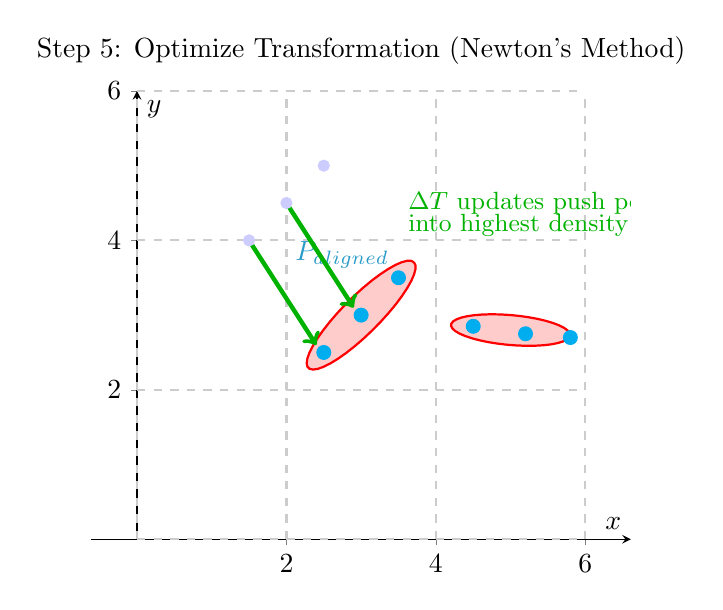
\begin{tikzpicture}
\begin{axis}[
    axis lines=middle,
    xmin=0, xmax=6, ymin=0, ymax=6,
    xtick={0, 2, 4, 6}, ytick={0, 2, 4, 6},
    axis equal, 
    xlabel=$x$, ylabel=$y$,
    title={Step 5: Optimize Transformation (Newton's Method)},
    grid=none
]

% Voxel Grid & Ellipses
\draw[black!20!white, dashed, thick, step=2] (0,0) grid (6,6);
\addplot[red, thick, domain=0:360, samples=40, fill=red!20!white] 
    ({3 + 1.0*cos(x)*cos(45) - 0.25*sin(x)*sin(45)}, {3 + 1.0*cos(x)*sin(45) + 0.25*sin(x)*cos(45)});
\addplot[red, thick, domain=0:360, samples=40, fill=red!20!white] 
    ({5 + 0.8*cos(x)*cos(-5) - 0.2*sin(x)*sin(-5)}, {2.8 + 0.8*cos(x)*sin(-5) + 0.2*sin(x)*cos(-5)});

% Final Aligned Source Point Cloud P' (cyan, nested in the dense probability zones)
\addplot[mark=*, cyan, only marks, mark size=2.5pt] coordinates {(2.5, 2.5) (3.0, 3.0) (3.5, 3.5)} node[anchor=south east, text=cyan!80!black] {\(P_{aligned}\)};
\addplot[mark=*, cyan, only marks, mark size=2.5pt] coordinates {(4.5, 2.85) (5.2, 2.75) (5.8, 2.7)};

% Highlight gradient ascent concept
\draw[->, green!70!black, ultra thick] (1.5, 4.0) -- (2.4, 2.6);
\draw[->, green!70!black, ultra thick] (2.0, 4.5) -- (2.9, 3.1);
\node[green!70!black, font=\small, anchor=west] at (3.5, 4.5) {\(\Delta T\) updates push points};
\node[green!70!black, font=\small, anchor=west] at (3.5, 4.2) {into highest density regions};

% Old points (faint)
\addplot[mark=*, blue!20!white, only marks, mark size=2pt] coordinates {(1.5, 4.0) (2.0, 4.5) (2.5, 5.0)};

\end{axis}
\end{tikzpicture}
\caption{Step 5: An optimization algorithm (typically Newton's Method) calculates the Hessian and gradient of the objective function to update the transformation parameters (rotation and translation). The source cloud "falls" into the high-probability valleys defined by the target's Gaussian mixture.}
\label{fig:optimization}
\end{figure}

\end{document}